% !TEX root = ../thesis.tex

\chapter{Polyhedra Analysis}
\mbox{}\\
\mbox{}\\
\mbox{}\\
Polyhedra analysis is one of the main tools of static analysis\cite{cousot1977abstract}. During the execution of a program variables can become bounded, either by numbers or by other variables. Polyhedrons are the most expressive ways of modelling all the different relations that can appear between a set of variables. Different alternatives exist for constraint representation instead of polyhedra, but none are as expressive. Unfortunately, it has worst case exponential space and time complexity meaning that using it on most real-world sized applications would very often cause it to either timeout or to run out of memory making it very impractical. Therefore, other domains have been more widely used such as octagon \cite{mine2006octagon}, zone \cite{mine2001new} or pentagon \cite{logozzo2010pentagons} , but all of these are less expressive and therefore less precise by design. In the recent years several techniques have been developed that have managed to speed up polyhedra analysis without the loss of precision\cite{gange2016exploiting,jourdan2017sparsity,marechal2017efficient}. We shall now briefly present some of these methods that are useful for this work.

\section{Polyhedra representation}
One of the technique used to increase the performance of static analysis involves the way in which we represent our domain\cite{singh2015making}. Polyhedra, for example, can be represented with both their constraint representation and their generator representation\cite{motzkin1953double} . To illustrate these different representations I will proceed with the following example. Lets assume we have the following set of commands:
\paragraph{Example 3.1}\mbox{}\\
\begin{center}
	$if \; x\geq0.5\wedge x\leq 1.5 \wedge y\geq 0.5 \wedge y \leq1.5: $\\
	$...\;\;\;\;\;$\\
	$end \qquad\qquad\qquad\qquad\qquad\qquad\qquad\qquad$
\end{center}

Inside of the if statement, the polyhedron would have the following shape:


\begin{center}
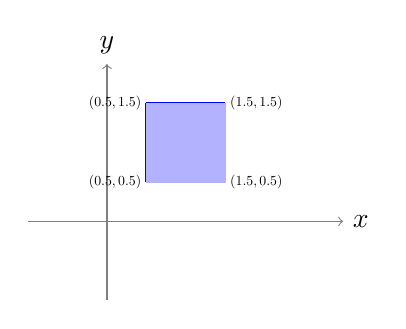
\begin{tikzpicture}
    \draw [thin, gray, ->] (0,-1) -- (0,2)      % draw y-axis line
        node [above, black] {$y$};              % add label for y-axis

    \draw [thin, gray, ->] (-1,0) -- (3,0)      % draw x-axis line
        node [right, black] {$x$};              % add label for x-axis

    \draw [draw=blue,thick] (0.5,0.5) -- (0.5,1.5)% draw the graph
   	 	node [left, black, scale =0.5] {$(0.5,1.5)$};
    \draw [draw=blue,thick] (0.5,1.5) -- (1.5,1.5)
    	node [right, black, scale =0.5] {$(1.5,1.5)$};
    \draw [draw=blue,thick] (1.5,1.5) -- (1.5,0.5)
    	node [right, black, scale =0.5] {$(1.5,0.5)$};
    \draw [draw=blue,thick] (1.5,0.5) -- (0.5,0.5)
    	node [left, black, scale =0.5] {$(0.5,0.5)$};
    	
    \draw [fill=blue!30,blue!30] (0.5,0.5) rectangle (1.5,1.5); 




\end{tikzpicture}
\end{center}
We can represent this information in two different possible ways.
\subsection{Constraint representation}
In constraint representation we model the polyhedron as the intersection of a finite number of closed half spaces and a finite number of subspace. The resulting polyhedron can be written as:

\begin{equation}
	P=\{x\in Q^n |Ax\leq b \wedge Dx=e\}
\end{equation}
where A,D are matrices and b,e are vectors of natural numbers. Therefore, the constraint representation of the above example would be:

\begin{equation}
	C = \{-x \leq -0.5,x\leq 1.5 , -y \leq -0.5 ,y\leq 1.5\}
\end{equation}

\subsection{Generator representation}
In order to encode a Polyhedron with the generator representation, we have to model it as the convex hull of three items: 

%TODO finish list with rep 
\begin{itemize}
	\item A finite set $V\in Q^n$ of vertices $v_i \in V$.
	\item A finite set $R \subseteq Q^n$ of rays. $r_i \in R$ are direction vectors of infinite edges of the polyhedron with one end bounded. The rays start from $v \in V$.
	\item  A finite set $Z \subseteq Q^n$ of lines. $z_i \in Z$ are direction vectors of infinite edges of the polyhedron with both ends unbounded. The lines pass through $v \in V$.
\end{itemize}
%TODO finish example
The result of generator representation on the previous example would have the following form: 
\begin{equation}
	G = \{ V = \{(0.5,0.5),(1.5,0.5),(1.5,1.5),(0.5,1.5)\}, R = \emptyset, Z = \emptyset \}
\end{equation}
\subsection{Polyhedra domain}

Now that we can represent our Polyhedra we can do some interesting calculations with them. The polyhedra abstract domain consists of the polyhedral lattice:
	$(P,\sqsubseteq,\sqcup,\sqcap,\perp,\top)$, and a set of operators that we can apply on them. The different operators are the following:
	\begin{itemize}
		\item Inclusion test: $P \sqsubseteq Q$
		\item Equality test: $P=Q$
		\item Join: $P\sqcup Q$
		\item Meet: $P\sqcap Q$
		\item Widening, this operator is applied to accelerate convergence since the polyhedral lattice has infinite height:
		\begin{center}
		  \[
    C_{P\nabla Q}=\left\{
                \begin{array}{ll}
                  C_Q $ if $P=\perp ;\\
                  C'_P\bigcup C'_Q, $ otherwise$;
                \end{array}
              \right.
  	\]
		
		\end{center}

		where $C'_p=\{c\in C_P |C_Q \vdash c \}$, and\\  $C'_Q=\{c\in C_Q |\exists c' \in C_P,C_P \vdash c $ and $((C_P\c')\bigcup \{c\})\vdash c' \}$
		where $C\vdash c$, test wether c can be entailed from constraints in C
		\item Conditional: let $\otimes \in \{\leq,=\},1\leq 1\leq n,\alpha \in Q$ then $\alpha x_i \otimes \delta$ adds the constraint $(\alpha-a_i)x_i \otimes\delta - a_i x_i$ to the constraint set C
		\item Assignement: $x_i = \delta$, first adds $x_i$ to P then augments C with $x_i -\delta = 0$
		
	\end{itemize}
	 In the following table we can see the respective complexities of the different operators according to the representation
	 
\begin{center}
\begin{tabular}{||c c c c||} 
 
 \hline
 Operator & Constraint & Generator & Both \\ [0.5ex] 
 \hline
 Inclusion $(\sqsubseteq)$ & $O(mLP(m,n))$ & $O(gLP(g,n))$ & $O(ngm)$ \\ 
 \hline
 Join $(\bigsqcup)$ & $O(nm^{2^{n+1}})$ & $O(ng)$ & $O(ng)$ \\
 \hline
 Meet $(\sqcap)$ & $O(nm)$ & $O(ng^{2^{n+1}})$ & $O(nm)$\\
 \hline
 Widening $(\bigtriangledown)$ & $O(mLP(m,n))$ & $O(gLP(g,n))$ & $O(ngm)$ \\
 \hline
 Conditional & $O(n)$ & $O(ng^{2^{n+1}})$ & $O(n)$ \\ 
 \hline
 Assignment & $O(nm^2)$ & $O(ng)$ & $O(ng)$ \\ 
 
 
 \hline
\end{tabular}
\end{center}
$m=|C|,g=|G|,LP(m,n)$ is the complexity of solving a linear program with m constraints and n variables\\
As we can see no representation is faster than the other, as some of the operators are quicker in one but others in the other. But, as we can see in the last table, when both representations are available all the operators are polynomial.\\
\paragraph{Chernikova's Algorithm} \mbox{}\\
 The first optimisation that one can do is to keep both representations of the the polyhedron and for each operator pick the representation that minimises the time complexity. A conversion between the two representations is possible thanks to Chernikova's algorithm\cite{chernikova1968algorithm}. 
 
 \section{Polyhedra Decomposition}
Another technique used to increase the efficiency of polyhedra analysis, is that of online decomposition \cite{singh2017fast}. It is based on the observation that during the execution of a program, not all it's variables are dependent on one another. Using this observation, we can separate the set of all variables into smaller, independent sets. Therefore, instead of having to represent the whole set of variables with one large polyhedron we can instead represent it with various smaller ones.\\ Let's assume we have a set of variables $\chi$ in a Polyhedron $P$. The set $\chi$ can be partitioned as $\pi_P=\{ \chi_1,\chi_2,..,\chi_r\}$, $\chi_i\subseteq\chi $. We call the partitioning of the set permissible iff $ \chi_i \cap \chi_j = \emptyset$, $ \forall i \neq j$. Once the decomposition has been done in this way, during the execution of an operator, it only has to be executed on the subset of blocks that contain it. This allows for a very large performance gain, giving us the following time complexity for the various operators.

\paragraph{Table 2} Asymptotic time complexity of Polyhedra domain operators with decomposition

\begin{center}
\begin{tabular}{||c c||} 
 
 \hline
 Operator & Decomposed  \\ [0.5ex] 
 \hline
 Inclusion $(\sqsubseteq)$ & $O(\sum_{i=1}^r n_ig_im_i)$\\ 
 \hline
 Join $(\bigsqcup)$ & $O(\sum_{i=1}^r n_i g_i m_i + n_{max} g_{max})$ \\
 \hline
 Meet $(\sqcap)$ & $O(\sum_{i=1}^r n_i m_i)$ \\
 \hline
 Widening $(\bigtriangledown)$ & $O(\sum_{i=1}^r n_i g_i m_i)$\\
 \hline
 Conditional & $O(n_{max})$ \\ 
 \hline
 Assignment & $O(n_{max}g_{max})$ \\ 
 
 
 \hline
\end{tabular}
\end{center}

 
\paragraph{Example 3.2} \mbox{}\\
Let's consider the with variables $X = \{x_1,x_2,x_3,x_4\}$ and $C = \{ x_1 + 2 \cdot x_3 \leq 10, x_2 = 1 \}$.\\
This polyhedron can be partitioned into three blocks $\pi_P = \{\{x_1,x_3\},\{x_2\},\{x_4\}\}$ and its corresponding factors are equal to:
\begin{center}
	$C_{P_1}\{x_1 + 2\cdot x_3 \leq 10 \} , C_{P_2}\{x_2 = 10 \}$
\end{center}

% TODO write example

\subsection{Decomposition operators}
As we change the model of our domains we must equally update the operators inside of these domains. For sake of brevity I will not go into detail about each of them, but I will only talk about the join operator as it plays an important role for this paper.\\
During the join of $P$ and $Q$, most of the time their factors will not be equal$(\pi_P \neq \pi_Q)$. Therefore, we have to remake their partitions in order for their factors to be equal $\pi = \pi_P\sqcup\pi_Q$. During most joins of a normal execution this will not cause much problem, but during some cases the join can merge all blocks producing the $\top$ partition. In order to rebuild the $\top$ partition from all its blocks we use the following formula:
\begin{equation}
	P = P_1 \Join P_2 \Join ... \Join P_r = (C_{P_1} \cup C_{P_2} \cup ... \cup C_{P_1}, G_{P_1} \times G_{P_2} \times  ... \times   G_{P_r})
\end{equation}
Due to the cartesian product, building the $\top$ partition can blow up the number of generators and therefore seriously slow down online decomposition.

\section{Reinforcement Learning for polyhedra analysis}
Both of the techniques presented in chapters 3.2 and 3.3, manage to achieve considerable performance gain without having to sacrifice any precision. Unfortunately, at some point compromises have to be made. Analysers that tune the precision and cost based on the program they are analysing are called parametric program analysers. Several such approaches already exist. \cite{oh2015learning,liang2011learning,heo2016learning} \\
As explained in 3.3.1. one bad constraint can significantly decrease the performance of the whole program. The trick is being able to identify this variable at the correct time. One of the explored solutions to this problem that we shall explore, is training a reinforcement learning algorithm  in order to decide when to apply abstractions \cite{singh2018fast}.\\
Intuitively, using reinforcement learning for polyhedra analysis seems quite straight. Let's imagine that for all the operators we have presented above, we have two versions of these $O_{pr}$ and $O_{pe}$. One of these is a slower and more precise operator and the other, using some sort of abstraction, is faster but not as precise. The goal of the reinforcement learning method would then simply be to select the correct operator at the right time, so that we get the most precise result in as little time as possible. Before this can be done, it is first necessary to initiate polyhedra analysis for reinforcement learning.

\subsection{Adapting polyhedra analysis for Reinforcement Learning}
As explained in 2.1., reinforcement learning uses a defined set of concepts. In some way, these concepts have to be translated into the domain of polyhedra analysis. A possible mapping can be done in the following way.
\begin{center}
\begin{tabular}{||c c||} 
 \hline
 RL concept & Polyhedra analysis concept  \\ [0.5ex] 
 \hline
 \hline
 Agent & Static analyzer\\ 

 State $s\in S$ & some features describing the polyhedron\\

 Action $a \in A$ & Abstract transformer \\
 
 Reward function r & some function representing the runtime\\
 
  & and precision of a polyhedron\\
 \hline
\end{tabular}
\end{center}
A more in-depth explanation of these concepts will come in the following chapter.

\subsection{Linear function approximation methods}
Existing methods already exploit this idea \cite{singh2018fast}. Using techniques such as Q-learning in order to learn their decision making policies. Q-learning is a common linear Q-function approximation technique and has shown some very good results when applied to the polyhedra domain.\\
However, recently, new reinforcement learning methods seem to be more focused on the use of nonlinear Q-function approximators, as they seem to give very good results on some  complex tasks. When the Q-function of the particular problem is nonlinear, Q-learning will never be able to learn the ideal policy. In these cases, deep Q-networks have a very real opportunity of exceeding the performance of the Q-learning based methods.\\
The use of nonlinear approximators has not yet been tested on the domain of static analysis. In the following chapters we shall explore the idea of using such methods in order to construct a new decision policy based on neural networks.
















